\documentclass[10pt]{article}

\usepackage[letterpaper,top=0.55in,bottom=0.64in,left=0.72in,right=0.72in]{geometry}
\usepackage{amsmath,amssymb,amsfonts}
\usepackage{booktabs}
\usepackage{graphicx}
\usepackage{xcolor}
\usepackage{microtype}
\usepackage{placeins}
\usepackage{caption}
\usepackage{enumitem}
\usepackage{times}
\usepackage{titlesec}
\usepackage{tikz}
\usetikzlibrary{arrows.meta,positioning,calc,fit}
\PassOptionsToPackage{hyphens}{url}
\usepackage{hyperref}
\usepackage[numbers,sort&compress]{natbib}

\hypersetup{
  colorlinks=true,
  linkcolor=blue!55!black,
  citecolor=blue!55!black,
  urlcolor=blue!55!black
}

\setlength{\columnsep}{0.24in}
\setlength{\parindent}{0pt}
\setlength{\parskip}{0.08em}
\setlength{\textfloatsep}{0.55em plus 0.2em minus 0.2em}
\setlength{\floatsep}{0.45em plus 0.2em minus 0.2em}
\setlength{\intextsep}{0.45em plus 0.2em minus 0.2em}
\setlist{nosep,leftmargin=*}
\captionsetup{font=small,labelfont=bf,skip=3pt}
\titlespacing*{\section}{0pt}{0.80em}{0.35em}
\titlespacing*{\subsection}{0pt}{0.55em}{0.20em}
\titleformat*{\section}{\large\bfseries}
\titleformat*{\subsection}{\normalsize\bfseries}
\AtBeginDocument{%
  \setlength{\abovedisplayskip}{0.36em plus 0.16em minus 0.12em}%
  \setlength{\belowdisplayskip}{0.36em plus 0.16em minus 0.12em}%
  \setlength{\abovedisplayshortskip}{0.18em plus 0.10em minus 0.08em}%
  \setlength{\belowdisplayshortskip}{0.26em plus 0.10em minus 0.08em}%
}
\emergencystretch=2em

\begin{document}
% Flush-left paragraphs with a soft ragged right edge; avoids forced long lines.
\raggedright
\twocolumn[{
% Title block intentionally follows the direct, compact structure of classic
% landmark neural-network papers: one problem, one method, one result.
\begin{center}
\rule{\textwidth}{1.35pt}
\vspace{0.12in}

{\LARGE\bfseries Paired-Acquisition Neural Factorization\\
for Computational Pathology\par}

\vspace{0.10in}
\rule{\textwidth}{0.50pt}
\vspace{0.14in}

{\bfseries Matthew Vaishnav}\par
Independent Researcher, Kitchener-Waterloo, Canada\par
\url{https://github.com/matthewvaishnav/paired-acquisition-factorization-scorpion}
\end{center}

\vspace{0.05in}
\begin{center}
\begin{minipage}{0.90\textwidth}
\begin{center}\bfseries Abstract\end{center}
\small
I trained a neural factorization model to separate biological tissue signal from scanner and acquisition signal using biology-preserving paired observations. The principal experiment uses 2,400 real histopathology images from 480 aligned regions on 48 human H\&E slides, each scanned on five devices. A frozen Paired-Acquisition Neural Factorization objective reduced biological scanner-probe accuracy from 0.7825 to 0.3989 on DINOv2 features while improving paired agreement and preserving near-perfect cross-scanner tissue retrieval. Without backbone-specific tuning, the same objective transferred to pathology-native Phikon and ImageNet ResNet50. Across the two unseen feature families, the slide-blocked scanner-probe difference was $-0.4019$ with 95\% bootstrap interval $[-0.4145,-0.3895]$, favorable on all 48 slides. Scanner identity remained strongly recoverable from a compact acquisition branch, indicating factor separation rather than representational erasure.

The method follows from two earlier failures. A locked adversarial study reduced site leakage but did not improve held-out tumor accuracy, and unconditional removal of a learned site component erased tumor-predictive information. Controlled latent-factor experiments then showed that ordinary observations and paired acquisitions are distinct resources. Under matched compute, doubling paired exposure improved recovery by $+0.037357$, while increasing unique anchors from 50 to 100 helped substantially more than increasing them from 100 to 200. Downstream PANDA, CAMELYON17, and PCam studies test whole-slide aggregation, institutional influence, external-center generalization, and systems constraints. The evidence supports a narrow conclusion: acquisition-associated information must be separated conditionally, with explicit protection of biology, rather than removed merely because it predicts site.
\end{minipage}
\end{center}
\vspace{0.08in}
}]

\section{Introduction}
Digital pathology representations contain more than morphology. Scanner optics, color response, compression, staining, preparation, local workflow, and institutional policy can all be encoded alongside tumor-relevant tissue structure. A representation may retrieve the correct specimen and support a downstream classifier while still making scanner or center identity easy to recover. Conversely, a method that suppresses every site-predictive direction can delete useful biology.

The central problem is therefore not ordinary domain invariance. It is \emph{conditional factorization}: acquisition-sensitive variation should become less recoverable from the biological representation, but tissue and diagnostic information must remain. This is difficult from ordinary observations alone because site and biology may be correlated. If a site-associated direction predicts tumor status, observational data cannot determine whether that direction is nuisance, biology, or an entangled mixture.

Biology-preserving acquisition pairs change the information structure. The same tissue region is observed under different scanners or acquisition states. What changes across a pair is candidate acquisition variation; what remains shared is candidate biology. Paired-Acquisition Neural Factorization uses this intervention structure to learn separate biological and acquisition branches and evaluates both what is removed and where it goes.

The specific contributions of this paper are as follows. First, I provide a locked negative-result sequence showing that lower site leakage alone does not imply better tumor prediction and that unconditional subtraction can erase biology. Second, I introduce a paired-acquisition factorization objective with explicit biological retention, acquisition prediction, reconstruction, variance control, and cross-factor decorrelation. Third, I evaluate the frozen objective on real paired scanner data with original-slide blocking and transfer it without retuning across three substantially different feature families. Fourth, I measure the separate roles of ordinary observations, unique paired anchors, and repeated paired exposure in controlled latent-factor experiments. Finally, I connect representation failure to later whole-slide and federated studies without using those studies to inflate the central paired-scanner claim. Focused companion PDFs carry exact protocols, frozen result tables, and reproduction scripts for study-specific claims.

\section{Linked Study Packages}
The public PDF is the research-program overview, not the complete protocol archive for every bounded claim. Study-specific repositories carry the exact preprocessing boundary, frozen split design, result tables, and reproduction scripts. I use logical method names in the text and repository-target slugs until public child-package URLs are verified.

\begin{table*}[t]
\centering
\caption{Focused study packages linked from the main research PDF.}
\small
\begin{tabular}{p{0.27\linewidth}p{0.46\linewidth}p{0.21\linewidth}}
\toprule
Package & What it contains & Repository status \\
\midrule
Paired-Acquisition Neural Factorization SCORPION core study & Primary paired-scanner method study on 48 original human H\&E slides, 480 aligned tissue regions, five scanners, and DINOv2/Phikon/ResNet50 transfer. & \href{https://github.com/matthewvaishnav/paired-acquisition-factorization-scorpion}{repository}; \href{https://matthewvaishnav.github.io/paired-acquisition-factorization-scorpion/paired-acquisition-factorization-scorpion.pdf}{PDF} \\
Paired-Acquisition Neural Factorization external canine SCC validation & Independent five-scanner canine SCC paired-acquisition validation on 805 geometry-qualified five-view regions from 44 biological samples. The locked projection reduced sample-blocked scanner-probe accuracy by 0.380 absolute while preserving same-region retrieval. & \href{https://github.com/matthewvaishnav/paired-acquisition-factorization-caninescc}{repository}; \href{https://matthewvaishnav.github.io/paired-acquisition-factorization-caninescc/paired-acquisition-factorization-caninescc.pdf}{PDF} \\
Paired-Acquisition Neural Factorization allocation study & Resource-allocation study testing biological pair diversity versus anchor repetition under matched pair-presentation budgets. The strongest allocation contrast was 200 versus 50 pairs at budget 6,400, with positive budget-doubling effects across allocations. & \href{https://github.com/matthewvaishnav/paired-acquisition-factorization-allocation}{repository}; \href{https://matthewvaishnav.github.io/paired-acquisition-factorization-allocation/paired-acquisition-factorization-allocation.pdf}{PDF} \\
\bottomrule
\end{tabular}
\label{tab:linked_study_packages}
\end{table*}

Verified study-package repositories and PDFs are linked from the public paper once the public URLs are live.



\section{The Data}
\subsection{SCORPION paired-scanner tissue}
The primary real-data study uses the public SCORPION benchmark \citep{ryu2025scorpion}. It contains 48 original human H\&E slides, ten aligned tissue regions per slide, and one image from each of five scanners for every region: AT2, GT450, DP200, P1000, and B300. The resulting dataset contains 480 biological regions and 2,400 images.

The original slide is the statistical unit. All regions and all scanner views from one slide remain in the same fold. Optimization seeds are averaged within slide before bootstrap and sign-flip inference. Patches, scanner views, regions, and repeated backbones are not treated as independent biological samples.

\subsection{Controlled latent-factor data}
Synthetic experiments generate known biological and acquisition factors, then mix them under controlled overlap and linear or nonlinear observation functions. Because the true factors are available, recovery can be measured using canonical correlation, Procrustes alignment, cross-factor leakage, paired invariance, counterfactual transport, and task retention. These experiments do not imitate the full complexity of histopathology; they isolate when the proposed supervision is sufficient or insufficient.

\subsection{Downstream pathology datasets}
PANDA supplies 10,611 verified slide-level Phikon feature bags for prostate grading and federated stress experiments \citep{bulten2022artificial}. CAMELYON17/WILDS supplies 455,954 examples from five centers for natural external-center validation \citep{bandi2018camelyon17,koh2021wilds}. PCam supplies a public patch-classification benchmark used for full-test, bootstrap, threshold, and simulated-site validation. These datasets test later levels of the learning pipeline; they are not substitutes for the paired-acquisition experiment.

\section{The Paired-Acquisition Neural Factorization Model}
\subsection{Paired acquisition supervision}
Let $x_{r,s}\in\mathbb{R}^{D}$ be the frozen feature for tissue region $r$ acquired by scanner $s$. A biology-preserving set contains several views of the same region:
\[
\mathcal{V}_r=\{x_{r,s_1},\ldots,x_{r,s_m}\}.
\]
The biological branch should be stable across members of $\mathcal{V}_r$, whereas the acquisition branch should retain information that distinguishes scanner states.

Under a simple latent model,
\[
x_{r,s}=Bz_{b,r}+Az_{a,s}+\varepsilon_{r,s},
\]
a paired difference cancels the shared biological term:
\[
x_{r,s'}-x_{r,s}=A(z_{a,s'}-z_{a,s})+(\varepsilon_{r,s'}-\varepsilon_{r,s}).
\]
The neural model does not assume the observation map is exactly linear, but the cancellation argument explains why paired observations contain information that ordinary site labels do not.

\subsection{Architecture}
For a standardized frozen feature $x\in\mathbb{R}^{D}$, Paired-Acquisition Neural Factorization uses two factor encoders, a joint decoder, and two scanner heads:
\begin{align}
 z_b &= f_b(x)\in\mathbb{R}^{d_b}, & d_b&=256,\\
 z_a &= f_a(x)\in\mathbb{R}^{d_a}, & d_a&=64,\\
 \widehat{x} &= g([z_b;z_a])\in\mathbb{R}^{D},\\
 \widehat{y}_{b} &= q_b(\operatorname{GRL}_{\gamma}(z_b)),\\
 \widehat{y}_{a} &= q_a(z_a), & \gamma&=1.
\end{align}
Both encoders are MLPs with hidden width 512:
\begin{align}
 h_c(x)&=\operatorname{LN}\{\operatorname{GELU}(W_{c,1}x+b_{c,1})\},\\
 f_c(x)&=W_{c,2}h_c(x)+b_{c,2},\qquad c\in\{b,a\}.
\end{align}
The decoder has widths $(d_b+d_a)\to512\to D$. The biological scanner head has widths $256\to128\to C$, the acquisition scanner head has widths $64\to64\to C$, and $C=5$ scanners. Gradient reversal is the identity in the forward pass and negates the encoder gradient:
\begin{equation}
 \operatorname{GRL}_{\gamma}(z)=z,
 \qquad
 \frac{\partial\operatorname{GRL}_{\gamma}}{\partial z}=-\gamma I.
\end{equation}
Thus $q_b$ predicts scanner identity while $f_b$ receives the opposite gradient; $q_a$ and $f_a$ minimize ordinary scanner cross-entropy. The architecture is therefore the factorization
\begin{equation}
 x\mapsto (z_b,z_a)=(f_b(x),f_a(x)),
 \qquad
 \widehat{x}=g([z_b;z_a]),
\end{equation}
where $z_b$ is optimized for same-region agreement and scanner suppression, and $z_a$ is optimized for scanner prediction and acquisition retention.

\subsection{Objective}
Let a minibatch be $\{(x_i,r_i,s_i)\}_{i=1}^{n}$, where $r_i$ is tissue-region identity and $s_i\in\{1,\ldots,C\}$ is scanner identity. Write $Z_b\in\mathbb{R}^{n\times d_b}$ and $Z_a\in\mathbb{R}^{n\times d_a}$ for the stacked factors, and let $u_i=z_{b,i}/\lVert z_{b,i}\rVert_2$. For anchor $i$, define $P(i)=\{p\ne i:r_p=r_i\}$ and
\begin{align}
 S_i &= \sum_{j\ne i}\exp(u_i^{\top}u_j/\tau),\\
 \ell_i &= -\frac{1}{|P(i)|}\sum_{p\in P(i)}
 \log\frac{\exp(u_i^{\top}u_p/\tau)}{S_i},\\
 \mathcal{L}_{\mathrm{pair}} &= \frac{1}{n}\sum_{i=1}^{n}\ell_i,
 \qquad \tau=0.1.
\end{align}
The reconstruction loss is the mean squared error
\begin{equation}
 \mathcal{L}_{\mathrm{recon}}
 =\frac{1}{nD}\lVert\widehat{X}-X\rVert_F^2.
\end{equation}
For $Z\in\mathbb{R}^{n\times d}$, define
\begin{align}
 v_j(Z)&=\frac{1}{n}\sum_{i=1}^{n}(Z_{ij}-\bar Z_j)^2,\\
 \ell_{\mathrm{var}}(Z)
 &=\frac{1}{d}\sum_{j=1}^{d}
 \left[1-\sqrt{v_j(Z)+\varepsilon}\right]_{+},
 \qquad \varepsilon=10^{-4},\\
 \mathcal{L}_{\mathrm{var},b}&=\ell_{\mathrm{var}}(Z_b),\qquad
 \mathcal{L}_{\mathrm{var},a}=\ell_{\mathrm{var}}(Z_a).
\end{align}
Let $Z_b^c=Z_b-\mathbf{1}\bar z_b^{\top}$ and
\begin{equation}
 C_b=\frac{1}{n-1}(Z_b^c)^{\top}Z_b^c.
\end{equation}
The within-biological covariance penalty is
\begin{equation}
 \mathcal{L}_{\mathrm{cov},b}
 =\frac{1}{d_b}
  \left\lVert C_b-\operatorname{diag}(\operatorname{diag}C_b)\right\rVert_F^2.
\end{equation}
The scanner losses are forward cross-entropies:
\begin{align}
 \mathcal{L}_{\mathrm{scan},b}
 &=-\frac{1}{n}\sum_i
 \log\!\left[\operatorname{softmax}
 \{q_b(\operatorname{GRL}_{\gamma}(z_{b,i}))\}\right]_{s_i},\\
 \mathcal{L}_{\mathrm{scan},a}
 &=-\frac{1}{n}\sum_i
 \log\!\left[\operatorname{softmax}\{q_a(z_{a,i})\}\right]_{s_i}.
\end{align}
Only the gradient entering $f_b$ is reversed.

Let $Y_s\in\mathbb{R}^{n\times C}$ be the one-hot scanner matrix. Column-standardize $Z_b$ and $Y_s$ using the same $\varepsilon=10^{-4}$ variance floor, producing $\widetilde Z_b$ and $\widetilde Y_s$. The direct scanner-dependence penalty is
\begin{equation}
 \mathcal{L}_{\mathrm{dep}}
 =\frac{1}{d_bC}
  \left\lVert
   \frac{1}{n-1}\widetilde Z_b^{\top}\widetilde Y_s
  \right\rVert_F^2.
\end{equation}
For $Z_a^c=Z_a-\mathbf{1}\bar z_a^{\top}$, the cross-factor penalty is
\begin{equation}
 \mathcal{L}_{\mathrm{xcov}}
 =\frac{1}{d_bd_a}
  \left\lVert
   \frac{1}{n-1}(Z_b^c)^{\top}Z_a^c
  \right\rVert_F^2.
\end{equation}
The frozen Paired-Acquisition Neural Factorization objective used in the five-fold and cross-backbone experiments is
\begin{align}
 \mathcal{L}
 &=\mathcal{L}_{\mathrm{pair}}
 +\mathcal{L}_{\mathrm{recon}}
 +\mathcal{L}_{\mathrm{var},b}
 +0.25\mathcal{L}_{\mathrm{var},a} \\
 &\quad
 +0.01\mathcal{L}_{\mathrm{cov},b}
 +0.5\mathcal{L}_{\mathrm{scan},b}
 +0.5\mathcal{L}_{\mathrm{scan},a} \\
 &\quad
 +20\mathcal{L}_{\mathrm{dep}}
 +0.05\mathcal{L}_{\mathrm{xcov}}.
\end{align}
The paired-consistency baseline is
\begin{equation}
 \mathcal{L}_{\mathrm{base}}
 =\mathcal{L}_{\mathrm{pair}}
 +\mathcal{L}_{\mathrm{recon}}
 +\mathcal{L}_{\mathrm{var},b}
 +0.01\mathcal{L}_{\mathrm{cov},b}.
\end{equation}
It shares the main retention and collapse controls but has no acquisition branch, scanner classifiers, direct scanner-dependence penalty, or cross-factor penalty.


\section{Preventing Representation Failure}
\subsection{Why site invariance was not enough}
The first Paired-Acquisition Neural Factorization study used a shared feature encoder, tumor head, and gradient-reversal site head. A locked confirmation reached approximately 0.9264 held-out tumor accuracy versus 0.9270 for the tumor-only baseline. The paired accuracy difference was approximately $-0.000625$ with an interval crossing zero. Site leakage decreased slightly, but the result was not a diagnostic-performance improvement.

A later factorized model separated diagnostic and site branches with reconstruction and covariance control. Validation selected the diagnostic-only baseline. An unconditional subtraction experiment was more decisive: the learned site-associated component remained strongly tumor-predictive, so subtracting it deleted useful biological signal. These failures define the design requirement for Paired-Acquisition Neural Factorization: removed information must be accounted for, and biology must be protected directly.

\subsection{Collapse and factor-retention controls}
A low scanner-probe score is meaningless if the biological branch is constant. Paired-Acquisition Neural Factorization therefore reports effective rank, per-dimension variance, tissue-region retrieval, paired cosine similarity, reconstruction, acquisition-branch scanner prediction, and acquisition-branch tissue retrieval. The desired pattern is not zero information everywhere. It is high tissue retention and reduced scanner recovery in biology, paired with high scanner recovery and substantially lower tissue retrieval in acquisition.

\subsection{Ordinary observations and paired resources}
The controlled program treats three quantities separately: ordinary observations $N_u$, unique paired anchors $N_p$, and paired repetitions $R_p$. Ordinary observations learn the task manifold. Unique anchors expose more biological locations under acquisition changes. Repetition supplies additional optimization signal for already observed interventions.

The pair-repeat experiments hold total paired presentations fixed while changing the allocation between $N_p$ and $R_p$. This distinguishes a true anchor-diversity effect from the simpler explanation that a model merely received more pair-loss updates.

\section{Details of Learning}
The frozen DINOv2 objective was selected through bounded calibration on development data, followed by independent-seed confirmation and final five-fold evaluation. The direct dependence weight of 20 was fixed before the final test stage. Cross-backbone transfer to Phikon and ResNet50 was preregistered before inspecting those outcomes. The transfer experiments used new shared seeds 701--705, the same rotating slide folds, and no backbone-specific objective or schedule changes.

Each SCORPION model used 75 epochs, region batch size 32, AdamW learning rate $3\times10^{-4}$, and weight decay $10^{-4}$. Every contrastive minibatch included all five scanner views of selected tissue regions. Inference used slide-block bootstrap intervals and sign-flip tests after averaging optimization seeds within each slide.

The pair-repeat synthetic study used overlap 0.975, nonlinear mixing, 320 optimizer steps, observational batch size 128, paired batch size 64, $N_u\in\{750,1500\}$, pair-consistency and hybrid-curriculum methods, and ten matched seeds. The two paired-presentation budgets were 6,400 and 12,800. Within each budget, the tested allocations were 50, 100, and 200 unique anchors with compensating repetition counts.

\section{Results}
\subsection{Frozen paired-scanner factorization}
Before Paired-Acquisition Neural Factorization training, scanner identity was strongly recoverable from all three feature families despite high tissue retention. The pathology-native Phikon representation had the highest baseline scanner-probe score.

\begin{table}[t]
\centering
\caption{Frozen representation audit before Paired-Acquisition Neural Factorization training.}
\scriptsize
\setlength{\tabcolsep}{2.6pt}
\begin{tabular}{@{}lccc@{}}
\toprule
Encoder & Cosine & Retrieval & Scanner \\
\midrule
ResNet50 & 0.8849 & 0.9550 & 0.7560 \\
DINOv2-B & 0.9851 & 0.9995 & 0.8400 \\
Phikon & 0.8787 & 0.9825 & 0.9640 \\
\bottomrule
\end{tabular}
\label{tab:frozen_audit}
\end{table}

On DINOv2, the frozen five-fold comparison reduced scanner-probe accuracy from 0.7825 to 0.3989, increased mean paired cosine from 0.8476 to 0.8789, and preserved mean tissue retrieval at approximately 0.9998.

\begin{table*}[t]
\centering
\caption{Paired-Acquisition Neural Factorization minus paired-consistency slide-blocked contrasts. Positive cosine and retrieval values and negative scanner-probe values are favorable.}
\small
\begin{tabular}{lrrrrr}
\toprule
Backbone & Scanner probe & Mean cosine & Worst cosine & Mean retrieval & Worst retrieval \\
\midrule
DINOv2-Base & $-0.3854$ & $+0.0310$ & $+0.0311$ & $-0.00008$ & $-0.00042$ \\
Phikon & $-0.4353$ & $+0.0900$ & $+0.0963$ & $+0.00060$ & $+0.00479$ \\
ResNet50 & $-0.3685$ & $+0.0255$ & $+0.0294$ & $+0.00808$ & $+0.01688$ \\
\bottomrule
\end{tabular}
\label{tab:crossbackbone}
\end{table*}

Both unseen backbones passed all seven preregistered criteria without retuning. Averaging Phikon and ResNet50 method differences within the same 48 slides gave scanner-probe difference $-0.4019$ with interval $[-0.4145,-0.3895]$, mean paired-cosine difference $+0.0578$ with interval $[0.0539,0.0615]$, and worst paired-cosine difference $+0.0628$ with interval $[0.0585,0.0672]$.

The acquisition branch retained scanner-probe accuracies of 0.8602, 0.9711, and 0.7845 for DINOv2, Phikon, and ResNet50, respectively. Its tissue retrieval was much lower than the biological branch: 0.1042, 0.0739, and 0.1705. Every biological dimension retained nonzero test-fold variance. The result is therefore consistent with separation, not a constant representation or simple information deletion.

\subsection{External paired-scanner validation package}
A companion external validation study applies the locked Paired-Acquisition Neural Factorization protocol to a public five-scanner canine squamous-cell-carcinoma dataset after geometry qualification. On 805 complete five-view regions from 44 biological samples, Paired-Acquisition Neural Factorization reduced sample-blocked scanner-probe accuracy from 0.7529 to 0.3614. The scanner-probe contrast was $-0.3803$ with bootstrap interval $[-0.3996,-0.3611]$, favorable in all 44 sample blocks, while same-region retrieval remained non-inferior. A later representation audit tested the branch-separation claim directly across folds 0--4 and seeds 911--915: scanner prediction fell from 0.878 in raw DINOv2 to 0.300 in the Paired-Acquisition Neural Factorization biological branch while same-region retrieval rose from 0.873 to 0.959; the acquisition branch retained scanner prediction at 0.968 while same-region retrieval fell to 0.031. Stronger linear, random-forest, kNN, and nonlinear MLP probes reproduced the same separation pattern. The exact dataset audit, P1000 orientation-normalization boundary, frozen encoder triage, five-fold result tables, and reproduction scripts are assigned to the companion \href{https://github.com/matthewvaishnav/paired-acquisition-factorization-caninescc}{repository} and \href{https://matthewvaishnav.github.io/paired-acquisition-factorization-caninescc/paired-acquisition-factorization-caninescc.pdf}{PDF}.

% External canine SCC representation-identifiability table.
% This file is included by paper/arxiv/main.tex and copied into the arXiv build.

\begin{table*}[t]
\centering
\small
\caption{\textbf{Paired-Acquisition Neural Factorization separates biological identity from acquisition identity.}
On an external multi-scanner canine SCC benchmark, raw DINOv2 features encode both scanner and biological identity.
Paired-Acquisition Neural Factorization produces a biological branch with low scanner decodability and high biological recoverability, and an acquisition branch with high scanner decodability and low biological recoverability.
Projected representations are summarized over folds 0--4 and seeds 911--915.}
\label{tab:paired_acquisition_figure1_benchmark}
\begin{tabular}{lrrrrrr}
\toprule
Representation & Runs & Scanner probe $\downarrow$ & Region R@1 $\uparrow$ & Sample R@1 $\uparrow$ & Eff. rank & Zero-var \\
\midrule
Raw DINOv2 & 1 & 0.878 & 0.873 & 0.986 & 442.802 & 0.000 \\
Paired reference & 25 & 0.746 & 0.940 & 0.999 & 186.481 & 0.000 \\
Paired-Acquisition Neural Factorization biological & 25 & \textbf{0.300} & \textbf{0.959} & \textbf{0.999} & 180.615 & 0.000 \\
Paired-Acquisition Neural Factorization acquisition & 25 & \textbf{0.968} & 0.031 & 0.421 & 47.355 & 0.000 \\
\bottomrule
\end{tabular}
\vspace{0.5em}

\begin{tabular}{llrrrr}
\toprule
Probe battery & Target & Raw DINOv2 & Paired ref. & Paired-Acquisition Neural Factorization bio. & Paired-Acquisition Neural Factorization acq. \\
\midrule
Linear/RF/kNN & scanner\_id $\downarrow$ & 0.662 & 0.573 & \textbf{0.255} & \textbf{0.971} \\
Linear/RF/kNN & sample\_id $\uparrow$ & 0.942 & 0.983 & \textbf{0.989} & 0.236 \\
MLP & scanner\_id $\downarrow$ & 0.832 & 0.740 & \textbf{0.207} & \textbf{0.972} \\
MLP & sample\_id $\uparrow$ & 0.940 & 0.977 & \textbf{0.986} & 0.326 \\
\bottomrule
\end{tabular}
\end{table*}


\subsection{Resource allocation under matched compute}
\begin{figure*}[t]
\centering
\resizebox{0.78\textwidth}{!}{% Pair-repeat Paired-Acquisition Neural Factorization resource-allocation figure.
% Black-and-white rendering designed for the compact main paper.
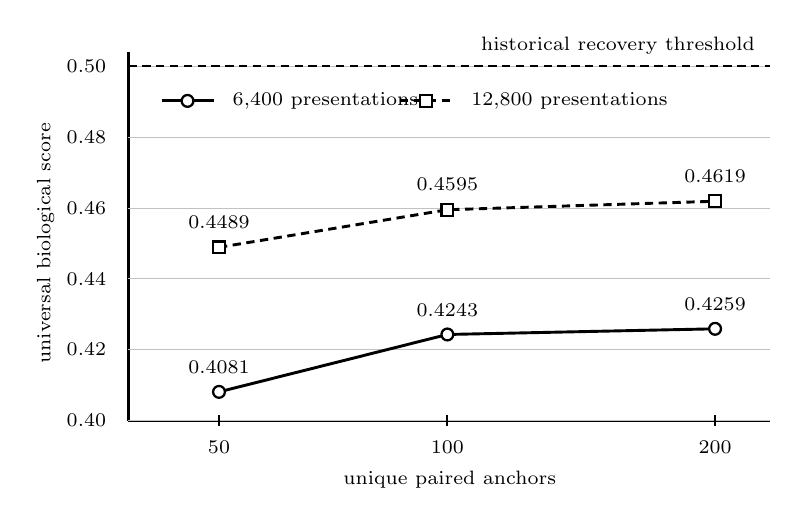
\begin{tikzpicture}[
  x=1cm,
  y=1cm,
  >=Latex,
  axis/.style={draw=black, line width=0.78pt},
  grid/.style={draw=black!24, line width=0.34pt},
  seriesa/.style={draw=black, line width=1.05pt},
  seriesb/.style={draw=black, line width=1.05pt, densely dashed},
  tick/.style={font=\scriptsize},
  legend/.style={font=\scriptsize, anchor=west}
]

% Plot area: x from 0 to 8.2; y=0 corresponds to score 0.40 and y=4.5 to 0.50.
\draw[axis] (0,0) -- (8.15,0);
\draw[axis] (0,0) -- (0,4.68);

% Horizontal grid and labels.
\foreach \yy/\lab in {0/0.40,0.9/0.42,1.8/0.44,2.7/0.46,3.6/0.48,4.5/0.50} {
  \draw[grid] (0,\yy) -- (8.15,\yy);
  \node[tick, anchor=east] at (-0.16,\yy) {\lab};
}
\node[tick, rotate=90, anchor=south] at (-0.82,2.25) {universal biological score};

% x ticks and label.
\foreach \xx/\lab in {1.15/50,4.05/100,7.45/200} {
  \draw[axis] (\xx,0.07) -- (\xx,-0.07);
  \node[tick, anchor=north] at (\xx,-0.13) {\lab};
}
\node[tick, anchor=north] at (4.08,-0.52) {unique paired anchors};

% Historical threshold.
\draw[draw=black, line width=0.64pt, dash pattern=on 3pt off 2pt] (0,4.5) -- (8.15,4.5);
\node[tick, anchor=south east] at (8.08,4.53) {historical recovery threshold};

% Legend, kept inside the unused upper-left region.
\draw[seriesa] (0.42,4.06) -- (1.08,4.06);
\filldraw[fill=white, draw=black, line width=0.82pt] (0.75,4.06) circle (0.075);
\node[legend] at (1.20,4.06) {6,400 presentations};

\draw[seriesb] (3.45,4.06) -- (4.11,4.06);
\draw[fill=white, draw=black, line width=0.82pt] (3.705,3.985) rectangle (3.855,4.135);
\node[legend] at (4.23,4.06) {12,800 presentations};

% 6,400 presentations: scores 0.4081, 0.4243, 0.4259.
\coordinate (a1) at (1.15,0.3645);
\coordinate (a2) at (4.05,1.0935);
\coordinate (a3) at (7.45,1.1655);
\draw[seriesa] (a1) -- (a2) -- (a3);
\foreach \p/\lab in {a1/0.4081,a2/0.4243,a3/0.4259} {
  \filldraw[fill=white, draw=black, line width=0.82pt] (\p) circle (0.075);
  \node[tick, anchor=south] at ($(\p)+(0,0.11)$) {\lab};
}

% 12,800 presentations: scores 0.4489, 0.4595, 0.4619.
\coordinate (b1) at (1.15,2.2005);
\coordinate (b2) at (4.05,2.6775);
\coordinate (b3) at (7.45,2.7855);
\draw[seriesb] (b1) -- (b2) -- (b3);
\foreach \p/\lab in {b1/0.4489,b2/0.4595,b3/0.4619} {
  \draw[fill=white, draw=black, line width=0.82pt] ($(\p)+(-0.075,-0.075)$) rectangle ($(\p)+(0.075,0.075)$);
  \node[tick, anchor=south] at ($(\p)+(0,0.12)$) {\lab};
}
\end{tikzpicture}
}
\caption{Pair-repeat allocation of unique paired anchors and repeated presentations. More total exposure produced the largest gain. Increasing unique-anchor diversity helped, with diminishing returns beyond approximately 100 anchors in the tested regime. No allocation crossed the historical 0.50 recovery threshold.}
\label{fig:resource_allocation}
\end{figure*}

At 6,400 paired presentations, the seed-blocked 200-versus-50 anchor contrast was $+0.017865$, with 95\% interval $[0.010560,0.026079]$, positive in all ten seed blocks, and exact two-sided sign-flip $p=0.001953$. The 200-versus-100 contrast was only $+0.001578$. At 12,800 presentations, the corresponding contrasts were $+0.013050$ and $+0.002422$.

Doubling paired exposure increased recovery by $+0.037357$ overall, with interval $[0.030315,0.043657]$, positive in all ten seed blocks, and exact $p=0.001953$. This establishes separate exposure and allocation effects. It does not establish a universal optimum or a recovered phase boundary.

\subsection{Whole-slide modeling on PANDA}
The whole-slide studies compare simple and learned aggregation under the same broad feature-bag setting. Mean-pooled Phikon plus an MLP reached validation QWK 0.7274. Gated AttentionMIL reached 0.8100. Three listed tuned TransnnMIL runs reached 0.8155, 0.8225, and 0.8086. An 18-run grid across six learning rates and three seeds reached a best mean validation QWK of $0.8257\pm0.0169$ at learning rate $10^{-4}$.

These results show a large improvement from mean pooling to attention-based MIL and establish a stable TransnnMIL training recipe. They do not yet prove architectural superiority over AttentionMIL, TransMIL, or nnMIL under fully matched compute.

\subsection{Federated site-signal auditing}
In the full-PANDA label-noise study, a tuned observable detector-switch policy kept clean performance effectively unchanged while improving global QWK by $+0.008009$ at 25\% dominant-site corruption and $+0.007482$ at 35\% corruption. A stronger transfer experiment froze a detector calibrated under label noise and applied it without retuning to systematic conservative ordinal threshold shift.

\begin{table*}[t]
\centering
\caption{Fixed detector transfer to conservative ordinal threshold shift. Deltas are detector-switch minus the clean-strategy baseline.}
\small
\begin{tabular}{rrrrr}
\toprule
Shift & Trigger & Global QWK $\Delta$ & Macro-F1 $\Delta$ & Worst-site QWK $\Delta$ \\
\midrule
0\% & 13.3\% & $-0.00025$ & $+0.00009$ & $+0.00151$ \\
25\% & 33.3\% & $+0.00129$ & $+0.00290$ & $+0.00353$ \\
35\% & 60.0\% & $+0.00542$ & $+0.00838$ & $+0.00991$ \\
45\% & 73.3\% & $+0.01053$ & $+0.01512$ & $+0.01290$ \\
\bottomrule
\end{tabular}
\label{tab:main_detector_transfer}
\end{table*}

At 35\% and 45\% shift, the bootstrap intervals for all three headline metrics were positive. Removing the most frequent diagnostic family reduced trigger rate but retained positive 35/45-shift means. In a 36-setting calibration-neighborhood sweep, 29 settings preserved low clean switching and positive 35\%/45\% gains across global QWK, macro-F1, and worst-site QWK.

CAMELYON17 then supplied natural center shift. With frozen ImageNet features, held-out-center accuracy was 0.8312 for FedAvg-style sample weighting, 0.9132 for equal-client weighting, and 0.9094 for dominant-source downweighting. With source-trained CAMELYON17 features, the corresponding accuracies were 0.9052, 0.9318, and 0.9322. FedAvg-style source-training accuracy reached 0.9991 in the latter study, showing that stronger source fit did not imply stronger unseen-center performance.

\subsection{Patch and systems studies}
On the full 32,768-example PCam public test set, the patch classifier reached 0.8526 accuracy and 0.9394 AUC; uncertainty was evaluated with 1,000 bootstrap resamples. Threshold analysis reduced missed tumor predictions by 61.7\% relative to the documented default operating point. Simulated-site PCam studies verified that equal, volume-based, and contribution-aware weighting implementations changed institutional influence on real image data, although patch-level performance was comparatively insensitive to those weight changes.

For the CAMELYON17 feature/head regime, 100 fp32 rounds across three clients were estimated at 24.98 GB for a full ResNet18 exchange versus 2.35 MB for a 512-to-2 head, a ratio of approximately 10,894. A coefficient-noise probe preserved the equal-client and downweighted advantages through noise standard deviation 0.20. A separate infrastructure simulation measured heterogeneous update times, dropout, failed rounds, and synchronous straggler burden. These are bounded systems studies, not formal privacy or hospital-deployment validation.

\section{Discussion}
The main result is not merely that a scanner classifier became worse. Scanner information remained strongly available in the acquisition branch, tissue identity remained almost saturated in biology, and the frozen objective transferred without retuning across a general self-supervised encoder, a pathology-native encoder, and a conventional ImageNet encoder. This pattern is difficult to explain as one-backbone overfitting or wholesale representational collapse.

The external canine SCC audit strengthens the same interpretation outside the primary human SCORPION benchmark. Across five folds, five seeds, and stronger probe families, the biological branch remained weakly scanner-decodable while retaining biological identity, and the acquisition branch remained strongly scanner-decodable while losing biological retrieval behavior. This is representation-identifiability evidence, not diagnostic validation, but it directly tests the central separation claim.

The negative studies are equally important. Gradient reversal changed leakage without improving tumor prediction. A factorized model did not beat its diagnostic-only baseline. Unconditional subtraction removed tumor-predictive information. Together, these findings reject a common shortcut: site predictability is not sufficient evidence that a direction is disposable.

The controlled resource experiments add a second result. Unique paired specimens and repeated pair presentations are not interchangeable, but neither is pair diversity the only resource. Over the tested range, doubling total exposure produced the largest improvement, moving from 50 to 100 anchors produced a meaningful additional gain, and moving from 100 to 200 produced only a small gain. This suggests that future real paired-acquisition collections should report both unique biological anchors and total paired exposure rather than calling both simply ``more paired data.''

The later PANDA, CAMELYON17, and PCam studies expose related authority problems at different scales. A pooling rule decides which patches dominate a slide. FedAvg decides that sample count controls institutional influence. Source-training accuracy can become nearly perfect while external-center accuracy remains worse. These studies do not validate one complete clinical system, but they show why representation, slide aggregation, institutional influence, and operational constraints must be audited separately.

The main limitations are clear. SCORPION contains 48 original slides and five scanners from one benchmark. Tissue retrieval is not a clinical endpoint. Linear probes cannot prove that every form of acquisition information has been removed; the canine stronger-probe battery reduces this concern but still cannot prove absolute independence. Synthetic recovery laws are local to the tested generator, metrics, and budgets. PANDA and CAMELYON17 results are retrospective and largely feature-level. Privacy-noise and infrastructure experiments are probes, not deployment guarantees. Companion PDFs provide exact study-specific boundaries so that external, canine, synthetic, whole-slide, and federated results are not collapsed into one clinical claim. No experiment establishes treatment benefit, prospective workflow safety, regulatory readiness, or universal biological--acquisition identifiability.

\section{Conclusion}
Biology-preserving paired acquisitions can supervise a neural factorization in which tissue identity is retained while scanner identity becomes substantially less recoverable from the biological branch. The same frozen objective transferred across DINOv2, Phikon, and ResNet50 on real human histopathology, while a compact acquisition branch retained scanner information. The external canine audit reproduced the branch-separation pattern across folds, seeds, and stronger probes. Earlier failures show why unconditional site removal is unsafe, and pair-repeat experiments show that unique anchors and repeated exposure are separate resources.

The broader research record extends this principle to slide aggregation, federated influence, external-center validation, and systems constraints. Focused companion PDFs now carry the detailed protocols and exact tables for bounded studies such as the external canine SCC validation. The supported claim remains bounded: acquisition-associated variation should be separated conditionally and audited explicitly, not erased merely because it predicts site.

\clearpage
\onecolumn
\appendix
\section{Complete Empirical Study Record}
The main text is deliberately narrow and result-first. The following appendix preserves the complete study-by-study research record, including methods, secondary experiments, negative results, systems probes, and claim boundaries.

\section{Broader computational-pathology study record}
The detailed SCORPION paired-scanner study above is the newest and strongest locked Paired-Acquisition Neural Factorization result, but it is not the whole research record. Earlier public PDF versions treated the repository as a three-level platform---representation, whole-slide aggregation, and institutional aggregation---and reported several distinct studies inside those levels. This section restores that study-by-study structure and adds the newer evidence without using one experiment to overstate another.

\subsection{Study map}
\begin{table}[!htbp]
\centering
\caption{Empirical studies represented in the public research record. Each row has its own unit of analysis and claim boundary.}
\small
\begin{tabular}{p{0.25\linewidth}p{0.20\linewidth}p{0.40\linewidth}}
\toprule
Study & Data or experimental substrate & Primary question \\
\midrule
Adversarial Paired-Acquisition Neural Factorization confirmation & Pathology-derived representations & Does lower site leakage improve tumor prediction? \\
Factorized and subtraction falsification & Pathology-derived representations & Can a learned site component be removed without deleting biology? \\
Synthetic two-resource phase maps & Controlled latent-factor generators & How do ordinary observations and paired interventions jointly control recovery? \\
Pair-repeat anchor allocation & Controlled nonlinear high-overlap regime & Under fixed paired exposure, how much does unique-anchor diversity matter relative to repetition? \\
PANDA baseline hierarchy & 10,611 verified Phikon feature bags & How much do mean pooling, gated attention, and TransnnMIL differ for whole-slide grading? \\
TransnnMIL stability grid & PANDA feature bags & Is the custom MIL model stable across optimization settings and seeds? \\
Dominant-site label-noise stress & PANDA-derived federations & When does sample-volume dominance become unsafe under controlled corruption? \\
Fixed detector transfer & PANDA-derived federations & Does a label-noise-calibrated detector transfer to systematic ordinal threshold shift? \\
Detector ablation and sensitivity & PANDA-derived federations & Is the detector dependent on one diagnostic family or one exact calibration? \\
CAMELYON17 external-center validation & 455,954 examples from five centers & Does sample-proportional source weighting generalize best to an unseen center? \\
CAMELYON17 center-subspace projection & CAMELYON17-trained features & Can source-center leakage be attenuated without collapsing tumor signal? \\
Communication accounting & CAMELYON17 feature/head regime & What communication burden is avoided by feature/head federation? \\
Privacy-noise stress & CAMELYON17-trained features & Do aggregation differences survive coefficient-noise perturbation? \\
Infrastructure-friction simulation & Three heterogeneous source-client profiles & How do speed, dropout, and stragglers affect practical federation? \\
PCam patch validation & Full public PCam test set & How well does the patch classifier perform, and how stable are its estimates? \\
PCam federated strategy probes & Real PCam patches split into simulated sites & Do institutional weighting strategies behave differently under balanced and heterogeneous partitions? \\
\bottomrule
\end{tabular}
\label{tab:study_map}
\end{table}
\FloatBarrier

\section{Earlier Paired-Acquisition Neural Factorization studies}

\subsection{Locked adversarial confirmation}
The first neural Paired-Acquisition Neural Factorization study used a shared feature encoder with a tumor head and a gradient-reversal site head. Development experiments suggested a small task improvement and reduced site leakage. A locked confirmation over new seeds did not reproduce the task advantage: the adversarial model reached approximately 0.9264 held-out tumor accuracy versus 0.9270 for the tumor-only baseline, a paired difference of approximately $-0.000625$ with an interval crossing zero. The site-probe difference was approximately $-0.003258$, with the paired bootstrap interval excluding zero.

The result therefore established a representation change, not a diagnostic-performance improvement. Lower recoverable site information was achievable, but it was not sufficient evidence that the representation had become more useful for tumor prediction.

\subsection{Factorized model selection and unconditional-subtraction falsification}
A later model used a shared stem with diagnostic and acquisition branches, reconstruction pressure, and cross-branch covariance control. Validation-based selection preferred the diagnostic-only baseline rather than the more elaborate factorized model. A subsequent subtraction experiment was more decisive: the learned acquisition-associated component remained strongly tumor-predictive, so removing it also removed useful biological information.

This falsified the simple rule that a direction should be deleted merely because it predicts site. The negative result directly motivated biology-preserving paired supervision and the later SCORPION study.

\subsection{Synthetic two-resource phase maps}
Controlled generators made the latent biological and acquisition factors known, allowing recovery to be measured rather than inferred indirectly. The experiments varied observational sample size $N_u$, unique paired-anchor count $N_p$, biological--acquisition overlap, linear versus nonlinear mixing, neural method, and seed. Pair-consistency, learned-operator, and hybrid-curriculum variants were evaluated using task retention, site leakage, cross-factor leakage, paired biological invariance, counterfactual transport, canonical-correlation recovery, and Procrustes recovery.

Under the compute-controlled high-overlap nonlinear protocol, sustained recovery boundaries were:
\begin{table}[!htbp]
\centering
\caption{Compute-controlled paired-anchor boundaries in the frozen synthetic follow-up.}
\small
\begin{tabular}{lrr}
\toprule
Method & $N_u$ & Sustained paired-anchor crossing \\
\midrule
Hybrid curriculum & 750 & 175 \\
Hybrid curriculum & 1500 & 150 \\
Pair consistency & 750 & 225 \\
Pair consistency & 1500 & 125 \\
\bottomrule
\end{tabular}
\label{tab:synthetic_boundaries}
\end{table}
\FloatBarrier

The threshold analysis used interval- and right-censored fits because some cells did not cross the historical recovery threshold within the tested intervention budget. The resulting relationship is a local, threshold-dependent empirical family: more observational data can reduce the paired-anchor requirement, while stronger overlap and nonlinear mixing increase it. It is not presented as a universal law.

\subsection{Pair-repeat anchor diversity versus repetition}
A separate allocation study fixed observational presentations, optimizer steps, pair-batch size, and total paired presentations while redistributing the paired budget between unique anchors and repetitions. The high-overlap nonlinear setting used $N_u\in\{750,1500\}$, pair-consistency and hybrid-curriculum methods, and ten matched seeds.

\begin{table}[!htbp]
\centering
\caption{Mean universal biological score across four method-by-$N_u$ strata under matched paired-presentation budgets.}
\small
\begin{tabular}{rrrr}
\toprule
Paired presentations & 50 anchors & 100 anchors & 200 anchors \\
\midrule
6,400 & 0.4081 & 0.4243 & 0.4259 \\
12,800 & 0.4489 & 0.4595 & 0.4619 \\
\bottomrule
\end{tabular}
\label{tab:matched_budget_means}
\end{table}
\FloatBarrier

At 6,400 presentations, the seed-blocked 200-versus-50 contrast was $+0.017865$, with 95\% bootstrap interval $[0.010560,0.026079]$, a positive difference in all ten seed blocks, and exact two-sided sign-flip $p=0.001953$. The 200-versus-100 contrast was only $+0.001578$. At 12,800 presentations, the corresponding contrasts were $+0.013050$ and $+0.002422$. Doubling total paired exposure increased recovery by $+0.037357$ overall, with interval $[0.030315,0.043657]$, positive effects in all ten seed blocks, and exact $p=0.001953$.

The supported interpretation is that total paired exposure was the dominant resource in this regime, unique-anchor diversity provided an additional benefit, and gains diminished beyond approximately 100 anchors. No allocation crossed the historical 0.50 recovery threshold, so this is an allocation and exposure result rather than a recovered phase boundary.

\section{PANDA whole-slide studies}

\subsection{Mean pooling, AttentionMIL, and TransnnMIL comparison}
The PANDA work studies weakly supervised prostate-cancer grading from whole-slide Phikon feature bags on the PANDA challenge data \citep{bulten2022artificial}. After HDF5 readability verification, 10,611 slide-level feature files were retained. Three principal model families were evaluated: a mean-pooled Phikon MLP, gated AttentionMIL \citep{ilse2018attention}, and TransnnMIL, a custom direction combining TransMIL-style correlated self-attention \citep{shao2021transmil} with nnMIL-style gated aggregation \citep{luo2025nnmil}.

\begin{table}[!htbp]
\centering
\caption{PANDA whole-slide validation evidence. QWK denotes quadratic weighted kappa.}
\small
\begin{tabular}{lr}
\toprule
Model or run & Validation QWK \\
\midrule
Mean-pooled Phikon + MLP & 0.7274 \\
Gated AttentionMIL & 0.8100 \\
Tuned TransnnMIL, seed 42 & 0.8155 \\
Tuned TransnnMIL, seed 123 & 0.8225 \\
Tuned TransnnMIL, seed 2025 & 0.8086 \\
\bottomrule
\end{tabular}
\label{tab:panda_model_hierarchy}
\end{table}
\FloatBarrier

The model hierarchy establishes that attention-based slide aggregation substantially improved on simple mean pooling in this feature-bag setting. TransnnMIL was favorable on two of three listed tuned seeds, but the margin over AttentionMIL remained small.

\subsection{TransnnMIL optimization-stability grid}
The stabilization study used the same 10,611 readable PANDA bags, three seeds, and six learning rates. The recipe used AdamW, warmup-cosine scheduling, two warmup epochs, gradient clipping at norm 1.0, and early stopping.

\begin{table}[!htbp]
\centering
\caption{TransnnMIL stability across three seeds per learning rate.}
\small
\begin{tabular}{lrrrr}
\toprule
Learning rate & Mean best val QWK & Std. & Min. & Max. \\
\midrule
$1\times10^{-4}$ & \textbf{0.8257} & 0.0169 & 0.8087 & 0.8425 \\
$2\times10^{-4}$ & 0.8245 & 0.0192 & 0.8077 & 0.8455 \\
$3\times10^{-4}$ & 0.8238 & 0.0160 & 0.8127 & 0.8422 \\
$5\times10^{-4}$ & 0.8158 & 0.0144 & 0.8042 & 0.8319 \\
$7\times10^{-4}$ & 0.8117 & 0.0163 & 0.7994 & 0.8301 \\
$1\times10^{-3}$ & 0.8160 & 0.0170 & 0.7998 & 0.8337 \\
\bottomrule
\end{tabular}
\label{tab:transnnmil_stability_full}
\end{table}
\FloatBarrier

This study supports optimizer stabilization and a wider usable learning-rate range. It does not yet establish that the complete TransnnMIL architecture is superior to simpler MIL methods under matched compute. Optional hierarchical, topology, and pruning branches remain separate implementation directions until controlled ablations validate them.

\section{PANDA federated site-signal studies}

\subsection{Dominant-site label-noise stress}
PathologyFL partitions PANDA-derived Phikon slide representations into simulated clients and applies label corruption only to the largest client. The study asks whether FedAvg's implicit rule---more samples means more influence---remains safe when sample volume and task-specific label signal diverge.

In the full-cache 15-seed study, a tuned observable switch kept FedAvg in the clean regime and moved to a 50\% cross-site blend when clean-calibrated diagnostics crossed a trigger threshold. Selected paired results were:
\begin{table}[!htbp]
\centering
\caption{Selected full-PANDA label-noise stress results for the tuned observable switch.}
\small
\begin{tabular}{rllr}
\toprule
Dominant-site corruption & Metric & Delta versus FedAvg & 95\% interval \\
\midrule
0\% & Global QWK & $+0.000126$ & $[-0.000144,0.000395]$ \\
25\% & Global QWK & $+0.008009$ & $[0.001345,0.014672]$ \\
35\% & Global QWK & $+0.007482$ & $[0.003919,0.011046]$ \\
45\% & Worst-site QWK & $+0.009713$ & $[-0.000257,0.019683]$ \\
\bottomrule
\end{tabular}
\label{tab:panda_label_noise}
\end{table}
\FloatBarrier

The clean false-switch rate was 6.7\%, while trigger rates increased strongly under 25--45\% corruption. The result supports a conditional stress-regime mechanism, not a universal replacement for FedAvg.

\subsection{Fixed detector transfer to conservative ordinal threshold shift}
A stronger transfer study froze one detector calibrated under dominant-site label noise and applied it without retuning to a systematic conservative ordinal threshold shift. The fixed rule used the 0.10 lower quantile, 0.80 upper quantile, at least three triggered diagnostic families, and no entropy diagnostic.

\begin{table}[!htbp]
\centering
\caption{Fifteen-seed fixed-detector transfer to conservative ordinal threshold shift. Deltas are detector-switch minus the clean-strategy baseline.}
\small
\begin{tabular}{rrrrr}
\toprule
Shift & Trigger rate & Global QWK $\Delta$ & Macro-F1 $\Delta$ & Worst-site QWK $\Delta$ \\
\midrule
0\% & 13.3\% & $-0.00025$ & $+0.00009$ & $+0.00151$ \\
25\% & 33.3\% & $+0.00129$ & $+0.00290$ & $+0.00353$ \\
35\% & 60.0\% & $+0.00542$ & $+0.00838$ & $+0.00991$ \\
45\% & 73.3\% & $+0.01053$ & $+0.01512$ & $+0.01290$ \\
\bottomrule
\end{tabular}
\label{tab:detector_transfer}
\end{table}
\FloatBarrier

At 35\% and 45\% shift, the bootstrap intervals for all three headline deltas were positive. The 25\% regime was directionally positive but inconclusive. The scientific value is transfer across stress mechanisms: the detector was calibrated under random label-noise stress and evaluated as frozen under systematic ordinal bias.

\subsection{Diagnostic ablation and calibration sensitivity}
The detector uses global QWK, worst-site QWK, site-QWK spread, mean absolute ordinal error, and severe-error rate. In the conservative-shift study, mean absolute error was the most frequent trigger, followed by worst-site and global-QWK degradation. Site spread alone was the weakest single-family variant.

Removing the strongest diagnostic family, \texttt{mean\_abs\_error\_high}, reduced the mean 35/45 trigger rate to 50.0\% but retained positive mean deltas of $+0.00701$ global QWK, $+0.01003$ macro-F1, and $+0.00856$ worst-site QWK. A 36-setting neighborhood sweep varied lower quantile, upper quantile, and minimum trigger count; 29 of 36 configurations preserved a clean trigger rate at or below 20\% and positive 35\%/45\% gains across all three headline metrics.

This study weakens the explanation that the transfer result is a one-feature shortcut or a single hand-picked calibration.

\section{CAMELYON17 external-center studies}

\subsection{Natural center-shift design}
CAMELYON17/WILDS provides natural hospital-center labels rather than only simulated client partitions \citep{bandi2018camelyon17,koh2021wilds}. The audited feature-level dataset contains 455,954 examples across five centers. Centers 0, 3, and 4 are source-training centers, center 1 is OOD validation, and center 2 is the held-out OOD test center.

\subsection{Frozen ImageNet ResNet18 feature study}
With frozen ImageNet ResNet18 features, FedAvg-style equal-patch weighting reached 0.8312 held-out test accuracy. Equal-client weighting reached 0.9132, an improvement of 8.20 percentage points, while downweighting the dominant source improved accuracy by 7.82 points. A validation-aware detector switch improved held-out accuracy by 6.58 points, and 43 of 112 detector settings were robust-positive in the threshold sweep.

\subsection{CAMELYON17-trained ResNet18 feature study}
A second study repeated the aggregation comparison using features from a source-trained CAMELYON17 ResNet18 checkpoint.

\begin{table}[!htbp]
\centering
\caption{Held-out center-2 accuracy under two feature families and three aggregation policies.}
\small
\begin{tabular}{lrrr}
\toprule
Feature extractor & FedAvg-style & Equal-client & Downweight dominant \\
\midrule
Frozen ImageNet ResNet18 & 0.8312 & 0.9132 & 0.9094 \\
CAMELYON17-trained ResNet18 & 0.9052 & 0.9318 & 0.9322 \\
\bottomrule
\end{tabular}
\label{tab:camelyon17_two_feature_studies}
\end{table}
\FloatBarrier

Under the source-trained representation, FedAvg-style weighting reached 0.9991 source-training accuracy while generalizing worse to center 2 than equal-client or dominant-source-downweighted weighting. The result supports the narrow observation that stronger source fit and sample-proportional influence do not automatically imply better external-center generalization.

\subsection{Paired-Acquisition Neural Factorization center-subspace projection branch}
A separate CAMELYON17 mechanism branch asked whether source-center information in the CAMELYON17-trained feature substrate could be attenuated without deleting tumor signal. Learned adversarial and subtractive variants did not materially reduce post-hoc center leakage. An explicit supervised center-subspace projection did: fitting a linear center classifier on an internal calibration split, removing the top right-singular directions of the centered classifier weight matrix, and probing on a separate internal split reduced center decodability while leaving tumor AUC essentially unchanged.

\begin{table}[!htbp]
\centering
\caption{CAMELYON17 center-subspace projection rank sweep. The effective center-discriminant rank is four after centering the five one-vs-rest class weight vectors.}
\small
\begin{tabular}{rrrr}
\toprule
Removed rank & Center accuracy & Tumor AUC & Tumor accuracy \\
\midrule
0 & 0.8946 & 0.9903 & 0.9550 \\
1 & 0.8530 & 0.9903 & 0.9564 \\
2 & 0.8256 & 0.9903 & 0.9564 \\
3 & 0.8092 & 0.9901 & 0.9562 \\
4 & 0.7636 & 0.9903 & 0.9560 \\
\bottomrule
\end{tabular}
\label{tab:camelyon17_center_projection}
\end{table}
\FloatBarrier

This is not a clinical-performance improvement claim and not complete source-center invariance. Its value is mechanistic: the adversarial variants failed, but a partially removable center-discriminant subspace exists and can be attenuated without collapsing the tumor probe.

\section{Federated systems stress studies}

\subsection{Communication accounting}
Communication was bounded for the CAMELYON17 feature/head regime. Under an explicit comparison with three source clients, 100 fp32 rounds, and a binary ResNet18 full-model proxy, full-model exchange was estimated at 24.98 GB. A 512-to-2 feature/head learner required approximately 2.35 MB, making the full-model proxy about 10,894 times larger.

Equal-client and dominant-source-downweighted policies used the same feature/head communication budget as FedAvg-style weighting, so their held-out-center gains were not purchased with additional traffic. A detector-style decision after 5, 10, or 25 rounds corresponds to estimated full-model communication reductions of 95\%, 90\%, or 75\% relative to 100 rounds. This is a bounded accounting result, not a measured wide-area hospital-network deployment.

\subsection{Privacy-noise robustness probe}
A coefficient-noise stress test used the CAMELYON17-trained ResNet18 features and added Gaussian perturbations to logistic-head coefficients at standard deviations 0.0, 0.01, 0.03, 0.05, 0.10, and 0.20, with five repeats per level. Equal-client and dominant-source-downweighted policies remained positive versus FedAvg-style weighting at every tested level. At noise standard deviation 0.20, the gains were approximately $+1.98$ and $+1.90$ percentage points.

This is not differential privacy, privacy accounting, membership-inference testing, or an update-inversion audit. It is a robustness probe under coefficient perturbation.

\subsection{Infrastructure-friction simulation}
A separate systems simulation modeled heterogeneous client speed, dropout, synchronous stragglers, an asynchronous proxy, communication cost, and detector-style reduced-round operation. The illustrative clients required 4, 7, and 13 minutes per local update. The outputs quantify wall-clock burden, failed rounds, straggler sensitivity, active-client counts, and traffic.

This study provides reproducible infrastructure accounting but is not a real hospital deployment benchmark. Containerized orchestration and measured network experiments remain future work.

\section{PCam validation studies}

\subsection{Patch-level classifier and uncertainty analysis}
The PCam study provides the repository's patch-level cancer-classification validation layer. The reported validation AUC was 0.9537. On the full 32,768-example public test set, the model reached 0.8526 accuracy and 0.9394 AUC. One thousand bootstrap resamples were used to report uncertainty.

A threshold and false-negative analysis examined screening-style operating trade-offs. In the documented analysis, threshold adjustment reduced missed tumor predictions by 61.7\% relative to the default operating point. This is retrospective benchmark analysis, not a prospective screening claim.

\subsection{Federated strategy probes on PCam}
Real PCam patches were also divided into simulated sites to exercise equal, volume-based, prestige-style legacy, and FAIR-WEIGHTS-H aggregation. The balanced benchmark completed without performance degradation from FAIR-WEIGHTS-H. Under heterogeneous simulated sites, the strategies produced different weighting trajectories, but patch-level performance was comparatively insensitive to those differences.

The value of this study is methodological: it verifies that the aggregation implementations run on real image data and that distinct policies actually alter institutional influence. It does not establish that FAIR-WEIGHTS-H improves clinical fairness or predictive performance.

\section{How the studies fit together}
The study sequence follows the learning pipeline:
\begin{itemize}[leftmargin=*]
  \item \textbf{PCam} establishes patch-level classification, uncertainty, and threshold-analysis infrastructure.
  \item \textbf{PANDA MIL} tests slide-level aggregation from pathology foundation-model feature bags.
  \item \textbf{Earlier Paired-Acquisition Neural Factorization} falsifies unconditional site removal and motivates paired supervision.
  \item \textbf{Synthetic Paired-Acquisition Neural Factorization} measures recovery when the ground-truth latent factors are known.
  \item \textbf{SCORPION Paired-Acquisition Neural Factorization} tests paired-acquisition separation on real human tissue across multiple representation families.
  \item \textbf{PANDA federated stress} audits sample-volume dominance under controlled label-process misalignment.
  \item \textbf{CAMELYON17} tests related aggregation hypotheses under natural held-out-center shift and tests whether explicit center-subspace projection can attenuate center leakage without collapsing tumor signal.
  \item \textbf{Communication, privacy-noise, and infrastructure studies} bound systems constraints without claiming that deployment is solved.
\end{itemize}

The integrated hypothesis is not that one architecture solves all of computational pathology. It is that representation formation, whole-slide aggregation, institutional influence, and systems constraints are separate failure surfaces that require separate experiments and explicit claim boundaries.


\section{Supporting Identifiability Calculations}
% This wrapper is copied into paper/arxiv/build by the PDF workflow.
\section{Paired-intervention identifiability calculations}
This section is a theoretical and synthetic extension motivating the next Paired-Acquisition Neural Factorization experiments. It is separate from the detector-switch evidence above and should not be interpreted as a clinical validation result.

\subsection{Why pairing changes the information structure}
Assume a pathology representation is generated by biological and acquisition factors:
\begin{equation}
  x=Bz_b+Az_a+\varepsilon.
\end{equation}
For a paired acquisition intervention preserving biology,
\begin{align}
  x_i&=Bz_{b,i}+Az_{a,i}+\varepsilon_i,\\
  x_i'&=Bz_{b,i}+Az'_{a,i}+\varepsilon_i'.
\end{align}
Subtracting gives
\begin{equation}
  \Delta x_i=x_i'-x_i=A(z'_{a,i}-z_{a,i})+(\varepsilon_i'-\varepsilon_i),
\end{equation}
so the shared biological term cancels. If acquisition latents have covariance $\Sigma_a$ and the noise is isotropic,
\begin{equation}
  \operatorname{Cov}(\Delta x)=2A\Sigma_aA^\top+2\sigma^2I.
\end{equation}
Thus the leading eigenspace of paired differences estimates the acquisition subspace. A first-order biological projection is
\begin{equation}
  P_{\perp A}=I-AA^\top,\qquad x_{\mathrm{bio}}=P_{\perp A}x.
\end{equation}

\subsection{Geometric overlap penalty}
Let $B$ and $A$ be orthonormal bases with canonical overlap $\rho$. Removing the acquisition subspace retains approximately
\begin{equation}
  E_{\mathrm{bio,retained}}\approx1-\rho^2.
\end{equation}
Hence $\rho=0.90$ leaves only $0.19$ of the biological energy outside the acquisition subspace, while $\rho=0.95$ leaves $0.0975$. Any component in $\operatorname{span}(B)\cap\operatorname{span}(A)$ is not uniquely assignable without additional assumptions.

\begin{table}[t]
\centering
\caption{Geometric difficulty proxy.}
\small
\begin{tabular}{ccc}
\toprule
$\rho$ & $1-\rho^2$ & $(1-\rho^2)^{-2}$\\
\midrule
0.50 & 0.7500 & 1.78\\
0.75 & 0.4375 & 5.22\\
0.90 & 0.1900 & 27.70\\
0.95 & 0.0975 & 105.19\\
\bottomrule
\end{tabular}
\end{table}

\subsection{Finite-pair sample complexity}
Let $m=pn$ be the number of paired examples, $D$ the observed dimension, and $\gamma$ the eigengap separating acquisition directions from noise. A Davis--Kahan-style perturbation argument suggests
\begin{equation}
  \sin\Theta(\widehat A,A)
  \lesssim
  \frac{C}{\gamma}
  \sqrt{\frac{D+\log(1/\delta)}{pn}}.
\end{equation}
Requiring this estimation error to be smaller than the surviving biological margin gives the provisional scaling prediction
\begin{equation}
  p_{\min}
  \gtrsim
  \frac{C^2(D+\log(1/\delta))}
  {n\gamma^2(1-\rho^2)^2}.
\end{equation}
This predicts diminishing returns in paired coverage, error decay proportional to $(pn)^{-1/2}$, and a sharp rise in required pairing as $\rho\rightarrow1$. The exact exponent and overlap dependence remain hypotheses rather than established theorems for the learned nonlinear models.

\subsection{Synthetic two-resource recovery boundary}
A follow-up synthetic phase-map study treated unpaired observations and paired interventions as distinct resources. It varied observational sample size $N_u\in\{500,1000,3000,10000\}$, high biological--acquisition overlap $\rho\in\{0.90,0.95\}$, linear versus nonlinear mixing, a grid of paired-anchor counts up to 300, five seeds, and pairing-aware methods. The endpoint $N_p^{\ast}$ was the smallest paired-anchor count at which the mean universal biological score crossed a predefined threshold and remained above it for every larger tested pair count.

At the primary sustained-recovery threshold $\tau=0.50$, 43 of 47 available conditions had observed boundaries and four were right-censored above the tested pair-count range. A model using $\log N_u$, overlap, and nonlinear mixing achieved the best leave-condition-out prediction and slightly outperformed a larger model with method-specific offsets.

\begin{table}[t]
\centering
\caption{Recovery-boundary model comparison at $\tau=0.50$. Lower leave-condition-out log RMSE is better.}
\small
\begin{tabular}{lc}
\toprule
Model & Log RMSE\\
\midrule
Power + overlap + nonlinearity & 0.455\\
Full model with method offsets & 0.459\\
Power only & 0.599\\
Constant boundary & 0.881\\
\bottomrule
\end{tabular}
\end{table}

The uncensored empirical fit was
\begin{align}
  \log N_p^{\ast}
  &=-1.568-0.659\log N_u \\
  &\quad+10.8792\rho+0.5345V,
\end{align}
where $V=1$ denotes nonlinear mixing and $V=0$ denotes linear mixing. Equivalently,
\begin{align}
  N_p^{\ast}
  &\approx0.208\,N_u^{-0.659} \\
  &\quad\times\exp(10.8792\rho)\exp(0.5345V).
\end{align}

An interval/right-censored likelihood fit used all 47 conditions and treated the four missing primary boundaries as exceeding the maximum tested pair count. It yielded
\begin{align}
  \log N_p^{\ast}
  &=-5.077-0.8086\log N_u \\
  &\quad+15.8347\rho+0.5277V,
\end{align}
and therefore
\begin{align}
  N_p^{\ast}
  &\approx0.00624\,N_u^{-0.8086} \\
  &\quad\times\exp(15.8347\rho)\exp(0.5277V).
\end{align}
The nonlinear multiplier is $\exp(0.5277)\approx1.695$. Within this tested synthetic regime, more observational data was associated with fewer required paired anchors, whereas overlap and nonlinear mixing increased the paired-anchor requirement.

The qualitative sign pattern was stable in ordinary least-squares sensitivity analyses at thresholds $0.45$, $0.50$, $0.55$, and $0.60$: the coefficient of $\log N_u$ remained negative, while the coefficients of overlap and nonlinear mixing remained positive. The number of observed boundaries decreased from 47 at $\tau=0.45$ to 27 at $\tau=0.60$, so stricter-threshold estimates are increasingly influenced by right censoring. Censored fits converged at $\tau=0.50$ and $\tau=0.55$; non-converged fits are not used as headline estimates.

These results support a threshold-dependent empirical family
\begin{equation}
  N_p^{\ast}(\tau)
  =C_{\tau}N_u^{-\alpha_{\tau}}
  \exp(\gamma_{\tau}\rho)
  \exp(\eta_{\tau}V),
\end{equation}
not a universal coefficient set. The raw-overlap term is a local approximation over the tested high-overlap range and does not by itself confirm the theoretical $(1-\rho^2)^{-2}$ dependence.

\subsection{Compute-controlled follow-up}
The fixed-epoch phase map coupled observational sample size to optimization exposure because larger datasets produced more minibatches per epoch. A follow-up protocol therefore fixed optimizer steps at $S=320$, observational batch size at 128, and one separate paired-supervision batch per optimizer step. It preserved held-out pairs for diagnostics and evaluated the harder unseen setting $\rho=0.975$ with nonlinear mixing across 20 seeds.

Under the predefined mean sustained-recovery rule, hybrid curriculum required 175 anchors at $N_u=750$ and 150 at $N_u=1500$. Pair consistency required 225 and 125 anchors, respectively. These point crossings were close to the threshold and should not be read as sharply identified constants.

A seed-cluster bootstrap produced broad, right-censored intervals. The median reduction was 25 anchors for hybrid curriculum and 50 for pair consistency, but both intervals crossed zero. The probability of a positive reduction was 0.564 and 0.670, respectively. These results are suggestive, not confirmatory.

The fixed-epoch relation remains a description of that training protocol, but recovery also depends on optimization exposure. A more complete resource description is
\begin{equation}
  \operatorname{Recovery}=f(N_u,N_p,R_p,S,\rho,V),
\end{equation}
where $R_p$ denotes paired-anchor repetition and $S$ denotes optimizer steps.

\subsection{Exact anchor diversity--repetition pilot}
A subsequent exact-schedule pilot separated unique paired anchors $N_p$ from presentations per anchor $R_p$. Every selected anchor appeared exactly $R_p$ times in a deterministic shuffled schedule. The pilot crossed $N_u\in\{750,1500\}$, $N_p\in\{50,125,225\}$, $R_p\in\{32,64,128\}$, two methods, and five new seeds, for 180 neural-network fits.

Increasing repetition improved the universal biological score in all 12 fixed-$(N_u,N_p,\text{method})$ slices. Increasing unique-anchor diversity also improved it in all 12 fixed-$(N_u,R_p,\text{method})$ slices.

\begin{table}[t]
\centering
\caption{Universal biological score at $N_p=225$ and $R_p=128$.}
\small
\begin{tabular}{lcc}
\toprule
Method & $N_u=750$ & $N_u=1500$\\
\midrule
Hybrid curriculum & 0.503 & 0.524\\
Pair consistency & 0.495 & 0.505\\
\bottomrule
\end{tabular}
\end{table}

Task AUC remained approximately $0.96$--$0.98$ while biological recovery, factor separation, and paired-invariance error changed substantially. Strong task prediction therefore did not certify a disentangled biological representation.

\subsection{Matched paired-supervision budgets}
To separate unique intervention diversity from repeated exposure, two exact-schedule experiments fixed total paired presentations within each budget while changing the allocation between $N_p$ and $R_p$. The first compared
\begin{equation}
50\times128=100\times64=200\times32=6400,
\end{equation}
with 100 pair-loss-active steps. The second doubled repetition at every anchor count,
\begin{equation}
50\times256=100\times128=200\times64=12800,
\end{equation}
with 200 pair-loss-active steps. Both experiments used the same 10 matched seeds, $N_u\in\{750,1500\}$, hybrid curriculum and pair consistency, 320 optimizer steps, and 40,960 observational presentations. Each budget therefore comprised 120 neural-network fits.

\begin{table}[t]
\centering
\caption{Mean recovery across four method-by-$N_u$ strata under matched paired-supervision allocations.}
\small
\begin{tabular}{rccc}
\toprule
Budget & $N_p\times R_p$ & Biological score & Factor separation\\
\midrule
6400 & $50\times128$ & 0.4081 & 0.7487\\
6400 & $100\times64$ & 0.4243 & 0.7626\\
6400 & $200\times32$ & 0.4259 & 0.7661\\
12800 & $50\times256$ & 0.4489 & 0.7874\\
12800 & $100\times128$ & 0.4595 & 0.7922\\
12800 & $200\times64$ & 0.4619 & 0.7987\\
\bottomrule
\end{tabular}
\end{table}

For global allocation contrasts, the four method-by-$N_u$ cells were first averaged within each seed, leaving 10 independent matched seed blocks. At 6400 presentations, 200 anchors exceeded 50 anchors by 0.0179 (95\% seed-bootstrap interval $[0.0106,0.0261]$), with a positive difference in all 10 seed blocks and an exact two-sided sign-flip $p=0.00195$. The 100-versus-50 contrast was also positive on average, but its interval included zero ($0.0163$, interval $[-0.0017,0.0328]$, $p=0.113$). At 12800 presentations, the 200-versus-50 contrast remained positive ($0.0131$, interval $[0.0015,0.0251]$), although the exact test was less conclusive ($p=0.0762$). The 100-versus-50 contrast was $0.0106$ ($p=0.195$).

Differences between 200 and 100 anchors were near zero at both budgets: 0.0016 at 6400 presentations and 0.0024 at 12800 presentations, with exact $p$-values of 0.822 and 0.607. The allocation result therefore indicates that concentrating all supervision on only 50 unique anchors is inefficient in this regime, while the incremental benefit beyond approximately 100 anchors is small and uncertain.

Doubling total paired exposure produced the larger and more reproducible effect. Averaged within each seed across all 12 matched cells, 12800 presentations improved the universal biological score over 6400 by 0.0374 (95\% seed-bootstrap interval $[0.0303,0.0437]$). All 10 seed blocks improved and the exact two-sided sign-flip test gave $p=0.00195$. The improvement was positive for each allocation separately: 0.0408 at 50 anchors, 0.0352 at 100 anchors, and 0.0360 at 200 anchors.

These controlled results identify total paired exposure as the dominant resource over this range, with a smaller diversity-allocation effect and diminishing returns between 100 and 200 unique anchors. No allocation mean at either budget crossed the predefined recovery threshold of 0.50, so the experiments characterize resource efficiency and response to supervision rather than a confirmed recovery boundary.

\subsection{Objective conflict in transport models}
For an operator trained with task, environment, reconstruction, transport, and consistency losses,
\begin{equation}
  \mathcal L=\mathcal L_{\mathrm{task}}+\lambda_e\mathcal L_{\mathrm{env}}+
  \lambda_r\mathcal L_{\mathrm{recon}}+\lambda_t\mathcal L_{\mathrm{transport}}+
  \lambda_c\mathcal L_{\mathrm{consistency}},
\end{equation}
the transport and consistency objectives may conflict. Their gradient cosine is
\begin{equation}
  G_{ct}=\frac{\nabla\mathcal L_c^\top\nabla\mathcal L_t}{\|\nabla\mathcal L_c\|\,\|\nabla\mathcal L_t\|}.
\end{equation}
A negative $G_{ct}$ indicates that reconstruction of acquisition-specific detail is opposing biological invariance.


% Render the complete existing bibliography in the focused PDF build.
\nocite{*}


\bibliographystyle{plainnat}
\bibliography{references}

\end{document}


